
Autonomic computing, a term introduced by IBM~\cite{computing2005architectural}, indicates systems that are
self-managing, self-tuning, self-healing, self-protecting, self-adapting, self-configuring, and self-organizing (briefly called self-* systems) \cite{babaoglu2005grassroots}. 
Some examples of IT related self-* areas of research targeted so far are:
adaptive parameter-level configuration management \cite{ensink2004coordinating, chang2000automatic, cangussu2004control},  
adaptive client-server communication \cite{loyall1998specifying, noble1997agile, balan2003tactics},  
adaptive resource allocation \cite{doyle_model-based_2003,lee1999scalable}, 
self-configuring network services \cite{huang2004building}, 
workload adaptive services \cite{menasce-accessing-ICAC-2004}, 
self-managing storage \cite{mesnier2004file}, 
statistical inference based decision-making management \cite{cohen2004correlating}, and
change and configuration management \cite{wang2003strider}. 

The portion of autonomic computing discipline that is relevant to our work is building self-managing complex resource sharing systems that manage themselves in accordance with high-level objectives specified by humans \cite{kephart_vision_2003}. Thus the autonomic aspect focuses on the fact that management is performed the systems themselves rather than being actively performed by human actors. However, this management should be according to objectives expressed by administrators. 
%
%%Mape loop .....
%At the heart of any autonomic system, there is an implicit or explicit feedback loop which 
%
%The man difference of autonomic management with tradtional computing system managements is the level of automation;
An autonomic manager usually understands the desired system objectives, matches those objectives with 
current or forecasted system behavior, and incorporates these into its decision governing the system. 

In terms of architecture, there is variety of ways for implementing autonomic management systems.
In the one focused in this research, adaptation strategies and mechanisms are separated from the applications or systems \cite{garlan2004rainbow, tesauro_utility_2004} (i.e. externalized adaptation). 
The architecture used is the well-known Monitor-Analyze-Plan-Execute (MAPE) loop suggested by IBM~\cite{computing2005architectural}  
where several components such as an analyzer, automated learner, forecaster, and a planner are used to decide about proper action(s) to be taken by actuators based on the current system measures. 
Figure \ref{fig:mapeloop}, adopted from \cite{mape-loop-pic}, presents a schematic structure of such loop.
In next sections, we describe the elements of autonomic computing loop in context of managing computer systems. 

% \section{Internalized and Externalized approaches to adaptation}
% \subsubsection{Internalized Approach}
% Autonomic systems can be built based on naturally occurring emergent systems (e.g. flocking\cite{spector2003emergence}, ant colonies \cite{camorlinga2004emergent}, and market economy \cite{kephart2001software,tesauro_utility_2004,eymann2003self}). 
%  Complicated patterns can emerge from the interplay large number of autonomous entities that behave according to some simple rules \cite{turing1952chemical, gierer1972theory}. 
% Feedback and reconfiguration can be done in these systems by incorporating evolution through the concept of death or failure (cells die, market actors  loose money).  
% 
% As an example of these systems, virtual markets, composed of numerous simple actors interacting with money, can be used to build complex goal-oriented decision support systems \cite{cheliotis2003autonomic}. For example, in a resource allocation problem in grid infrastructure \cite{foster1997globus,foster2002grid} market-based control can be applied to remove unwanted resource contention. 
% \cite{montresor2003messor} showed how an ant algorithm could be used to solve the problem of dispersing tasks uniformly over a network. Similarly, the Routing Information Protocol (RIP) routing table update protocol uses simple local rules that result in good overall routing behavior. Other examples include autonomous grid scheduling protocols \cite{kreaseck2003autonomous} and peer-to-peer file sharing networks [gnutella, stoica2001chord]. 
% In all of these systems the whole has a functionality more than the sum of the parts.
% 
% %Assume the Grid manager has to decide about the hosts that should handle tasks based on the resources left on the host (i.e. central processing unit (CPU), network and disk interfaces, and data storage) and the nature of the tasks. In market oriented approach, one can assign tasks to autonomous entities and letting these entities find a suitable host. autonomous entities have to use electronic currency to purchase the resources necessary to complete its task. based on the resource usage at hosts, market determines prices for that host (i.e. congestion results in high prices). Less congestion through even  spatial distribution of agents will follow naturally as agents choose hosts with lower prices. Temporal load balancing will be also resulted from the fact that some agents wait until prices drop. 
% 
% \subsubsection{Externalized approach}

% \begin{figure}[hb]
% 	\centering		
% 	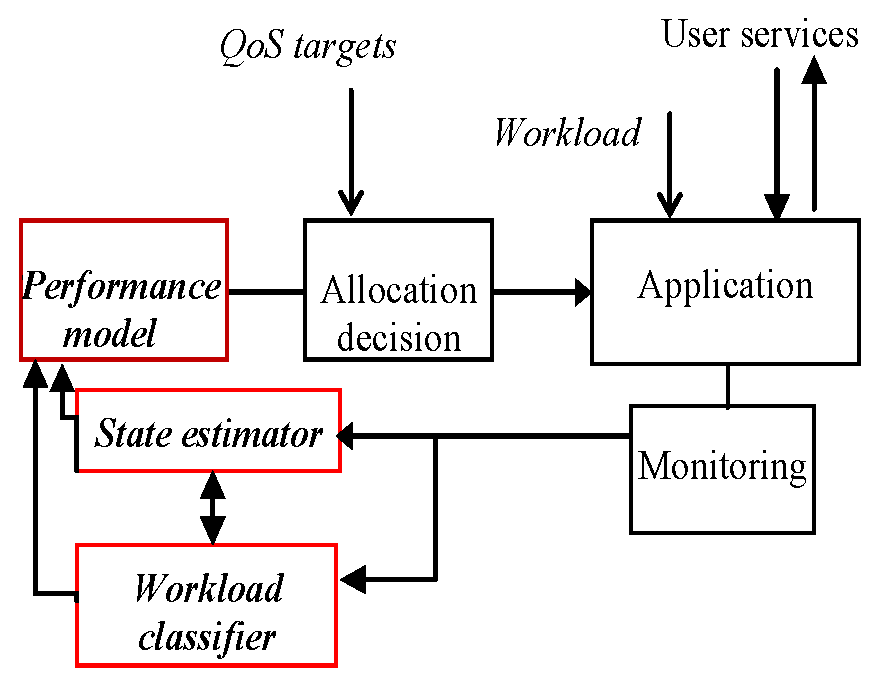
\includegraphics[width=0.45\textwidth]{image/autonomic-loop.eps} 
% 	\caption{Architecture of an autonomic loop based control.} 
% 	\label{fig:fig1}
% \end{figure}
\begin{figure}
	\centering		
%	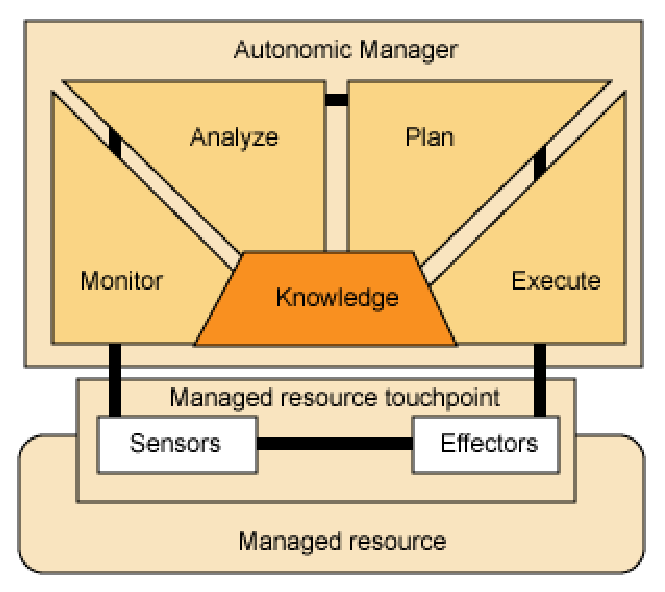
\includegraphics[width=0.45\textwidth]{image/mapeloop.eps} 
% 	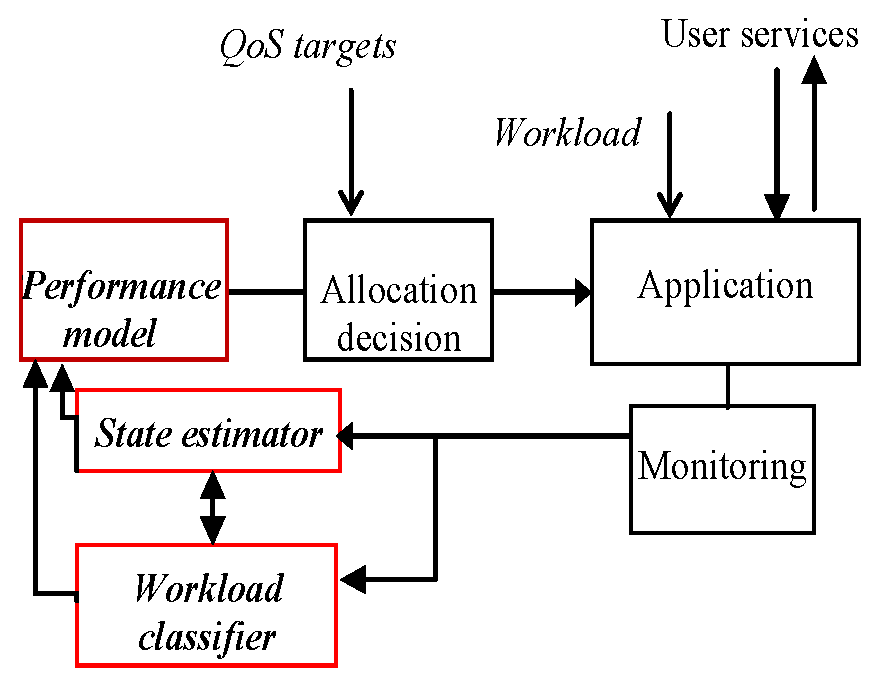
\includegraphics[width=0.45\textwidth]{image/autonomic-loop.eps} 
	\caption{Architecture of autonomic management suggested by IBM.} 
	\label{fig:mapeloop}
\end{figure}

% 
% 
% Controllers may vary in their architectural complexity. 
% The nature of performance criterion function, weather it has set point nature (e.g. $\text{minimize}(\Sigma (a_s-a_t))$) or optimization nature (e.g. $\text{maximize}(\Sigma profit_t$)), is an important factor in complexity of the controller. 
% The primary use of a feedback loop is to satisfy a constraint or guarantee an invariant on the outputs of the system under control over time. As an example of this, is a controller to satisfy the invariant that CPU utilization should be less than $U_0$, or that the response time should be below $R_0$. 
% Another usecase for a feedback loop is to optimize an objective function over time.
% An example for optimization based feed-back loops is a controller that aims to minimize CPU power consumption of a web server while keeping the request buffer under a certain size.
% Such a loop, for instance, can be used to maintain high server utilization while avoiding overload. 
% More complex cases of feedback based loop can incorporate planning. In the following subsections we briefly mention the related work using each of these types of feedback loops. 
% Complexity of a controller also depends on the existence of a model for the target system, the theory underpinning the model, and the usage (or omission) of an estimator to track hidden variables in the model. 

\section{Monitoring}
Monitoring subsystem is responsible for measuring inputs, and outputs of the managed system, quantifying them, sometimes aggregating them, and keeping them as a history. 
Another feature of a complete monitoring system would be to send notifications to inform the administrator or autonomic manager about an important condition (e.g. high CPU load, full memory, or a failed health check) using the network. These conditions can be user-defined and based on performance values breaching certain thresholds. 
The monitoring data will be processed in subsequent autonomic management subsystems and eventually makes its way into decisions taken by the autonomic manager. 

In computer systems, from performance point-of-view, there are several metrics to be monitored.
For example, in a typical transactional system one can use hardware level metrics of each host, 
operating system metrics (e.g. file, network, and memory management subsystems) of each virtual machine, 
process level metrics, and service specific metrics for different types of server processes (e.g. load balancer, web server, application server, and database server). 
In a batch oriented system, in addition to hardware and OS level metrics, metrics such as the average number of jobs in the job queue or average job's queuing time also exist.  
Table \ref{tab:alerts-metrics} summarizes these metrics.

There are several existing tools for monitoring computer systems.
\textit{Collectd}~\cite{collectd} is a monitoring daemon for collecting system performance statistics. It accepts plug-ins for collecting new types of metrics.
\textit{Nagios}~\cite{nagios} is another powerful industry level tool for monitoring entire IT infrastructure.
Java Management Extensions (JMX)~\cite{jmx} technology included in the Java SE platform provides a generic standard for publishing and using the data of monitoring devices especially Java base web and application containers. 

\begin{table*}[h]
    \centering
    \begin{tabularx}{\linewidth}{ r X }
    %\begin{tabular*}{0.90\textwidth}{|l|l|}
    \hline \\
    Alert Target & Metrics \\ \hline \\
    Hardware & CPU utilization, disk access, network interface access, memory usage \\
    General OS Process & cpu-time, pagefaults, real-memory (resident set) size \\
    Load balancer & request queue length, session rate, number of current  sessions, transmitted bytes, num of denied requests, num of errors \\
    Web server & transmitted bytes and requests, number of connections in specific states (e.g. closing, sending, waiting, starting, ...) \\
    Application server & total threads count, active threads count, used memory, session count \\
    Database server & number of active threads, number of transactions in (write, commit, roll-back, ...) state \\
    Message Queue & average number of jobs in the queue, average job's queuing time \\
    \hline \\
    \end{tabularx}
  \caption{List of the metrics used in defining autoscaling alerts.}
  \label{tab:alerts-metrics}
\end{table*}


\section{Analyzing} 
\input{online-estimation.tex} 


\section{Planning and Feed-forward Predictive Control} 
 \label{sec:optimizers} 
In general the goal of any optimal control approach is to choose a sequence of feasible \textit{control actions} that maximizes a defined \textit{performance criterion} (or objective function)\footnote{One can instead say optimal control minimizes an expected total cost function}. % or simply regulates the system towards an objective. 
The analyzer components (described in the past section) provides an accurate model that can be used 
in calculating the cost and performance criterion by providing projection of system's behavior and state in the future. 
%(as opposed to \textit{regulators}), because of use of  complex goals and objective functions, the simple schema of simply feeding back control error (like classical linear continuous proportional-integral (PI) controllers) might not be possible. 
A planner uses this comprehensive and accurate model to rapidly explore multiple decisions and find near-optimal solution during each  step \cite{litoiu_hierarchical_2005,aiber2004autonomic} (see Figure \ref{fig:optimization-based-planner}). 
% Autonomic self-optimization according to business objectives is also studied in \cite{aiber2004autonomic},
In context of control theory, this schema is called open-loop or feed-forward predictive control. 
% Since such open-loop control cannot compensate for disturbances or noise that is not mentioned in the model, the guarantee of a system's good performance is the accuracy of the model. 
%The model in this scheme should take into account reference and disturbance inputs and be tuned to stay accurate. 
% Modeling the system to well-known queuing theory and estimating the parameters of such model is also a common practice. 
In the next subsections we describe two common approach currently used in planning and optimization for systems performance. 
\begin{figure}[h]
	\centering
	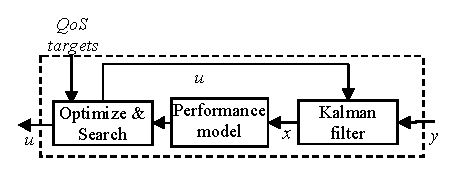
\includegraphics[width=0.45\textwidth]{image/loop/controller-optimizer.eps}
	\caption{Structure of an optimization based planner.}  %subref{fig:1}
	\label{fig:optimization-based-planner}
\end{figure}
 
% \subsection{Optimization of steady-state models}
\subsection{Searching in continuous space}
\label{sec:static-optimizer}
If one can describes the objectives of controller in terms of outputs of an identified system model (e.g. performance, QoS or profit), the proper control inputs that satisfy the objectives can be easily derived by searching the space formed by choosing actions and applying them to the model.
In case the search can be converted into classical mathematical optimization problem, several approaches such as primal decomposition, interior point methods, simulation annealing, etc can be used to derive the proper control inputs. 
% Algorithm~\ref{algorithm1} represents the primal method for soling constraint optimization problems. 
Usually optimizer takes initial control inputs, the number of iterations during optimization, the utility model, and a set of constraints as input
and outputs optimal control values and maximum utility gained from those. This process is usually done iteratively.
To skip falling into local optimums global optimization techniques can be utilized. 

Although simple, the applicability of this form of search is reduced when the system model is discrete or time-varying. In the following subsection, planning for such models is explained. 

% \begin{algorithm}[!h]
% 	\small
% 	\SetAlgoVlined
% 	\SetKwInOut{Input}{input}
% 	\SetKwInOut{Output}{output}
% 	\SetKwInOut{Initialize}{initialize}
%   \SetAlFnt{\tiny}
% 
% \Input{initial control values, utility model, a set of constraints}
% \Output{optimal control values, maximum utility}
% \BlankLine
% \While { $k < k_{\text{max}}$}
% {
% 	compute value of each constraint $U_i$.\nllabel{al1-step_1}
% 	\BlankLine
% 	
% 	\If {no constraint is violated, move towards optimum: $(max(U_i(A))>0)$ }
% 	{
% 		compute global utility function.\nllabel{al1-step_2.1} 
% 		\BlankLine
% 
% 		record the global maxima.\nllabel{al1-step_2.2} 			
% 		\BlankLine
% 
% 		calculate objective function's subgradient.\nllabel{al1-step_2.3} 	
% 		\BlankLine
% 
% 		move towards subgradient and the optimum. \nllabel{al1-step_2.4}			
% 		\BlankLine
% 	}
% 	\ElseIf{there is some violated constraint}{
% 
% 	  find most violated constraint. \nllabel{al1-step_3.1}
% 	  \BlankLine
% 
% 		compute the subgradient value of most violated  constraint. \nllabel{al1-step_3.2}  
% 		\BlankLine
% 
% 		select step size.\nllabel{al1-step_3.3}
% 		\BlankLine
% 
% 		move away from subgradient and the optimum. \nllabel{al1-step_3.4}
% 		\BlankLine
% 	}
% 	project each individual variable based on its local constraint. \nllabel{al1-step_4}  		
% 	\BlankLine
% 
% 	$k = k + 1$\; 	
% 	\BlankLine      
% }
% \caption{A centralized solution for the problem using primal method. }  
% \label{algorithm1}
% \end{algorithm}

\subsection{Searching in discrete space}
% \subsection{Searching through time-varying models} 
% Regulators described in subsection \ref{sec:regulators} usually assume a linear model for system dynamics with an unconstrained state space, and a continuous I\/O domain.
% The goals targeted by those are also usually just simple set-pointing. 
 % address some limitations of classical control techniques for non-linear systems and complex goals (e.g. multiple QoS goals). 
In many cases, an autonomic system designer deals with a discrete model that varies over time.  
The most commonly known tool that makes use of such model is a Limited lookahead controller (LLCs) \cite{abdelwahed2004control, kandasamy2004self}.       
It explores a search space formed by different choices of control actions (while control inputs must be chosen from a finite set) over the predicted model \cite{bhat2006enabling} to find the optimal solution; thus, management problem is posed as a sequential optimization under uncertainty. 
Compared to steady-state optimization approach studied in subsection \ref{sec:static-optimizer}, LLCs use time-varying models that take into account the transient behavior of the system such as steady-state formulation of equation \ref{eq:generic-state-space-equation}.
However, control inputs $u(k)$ are chosen from a finite set of control options available $U(x)$ \footnote{The finite set of all permissible control inputs can be denoted as $U$.} at the corresponding system state $x$.
Here systems' state space $X$ is defined by operating constraints described by the inequality $H(x) \leq 0$.

The objective of control, which is encoded as transient cost or utility using norm-based function, implicitly defines desired state and preferable paths toward this state:
\begin{equation} \label{eq:llc-cost-general}
J(x(k), u(k),\Delta u(k)) = \alpha_1. ||x(k) - x^*||+\alpha_2.||u(k)||+\alpha_3.||\Delta u(k)||	
\end{equation}
here $x(k)$ is the current state, $u(k)$ denotes the control inputs, $\Delta u(k)$ denotes the corresponding change in these inputs, 
and $\alpha_1$, $\alpha_2$, and $\alpha_3$ are user-defined weights denoting the relative importance of the variables in the cost function.

According to feed-forward controller scheme, the controller explores a set of future states within the lookahead horizon, 
At every predicted state, environmental inputs to the controller must be predicted and different choices of control inputs should be navigated.
Controller then selects a path that minimizes the cumulative cost while satisfying both state and input constraints within lookahead horizon
$u^*(j)|j\in [k +1, k + N]$: 
\begin{equation} 
  \begin{split}
    \text{compute: } & \text{min}_U \sum_{j=k}^{k+N} J(x(j),u(j))  \\
    \text{subject to: } 
%    & \hat{\omega}(j)=\phi(\underline{\omega}(j-1),a(j)) \\
    & H(f(x(j),u(j),\hat{\omega}(j)))\leq 0 \\
    & u(j)\in U(x(j))
  \end{split}
\end{equation}
The first control input leading to this path is chosen as the next control action.

%number of navigated states within prediction horizon $N$ would be $\sum_{i=1}^N |U|^i$ where $U$ is the number of available choices. 
                                                                               
% \paragraph{Example 1. Control of Data Streaming}
% Consider the problem transferring data between two clusters (e.g. data generator cluster and analysis cluster) using a
% data transfer cluster which is located between these two and is composed of $n$ servers.
% 
% Data transfer cluster tries to transfer as much of the generated data as possible to the remote cluster
% for analysis ($\mu_i(k)$ denotes the data transfer rate over the network link) depending on the rate and volume of data generated by the first cluster ($\lambda_i(k)$ denotes the data generation rate by data generation cluster) and the available network bandwidth $B(k)$ to send to the second cluster.
% If the available network bandwidth is insufficient or network interfaces are saturated it will use the local hard-disk storage as a temporary buffer. In this scenario We need a controller that avoids saturation of network interface buffer of data transfer nodes by transferring extra data to hard-disk when necessary (assume $\gamma_i(k)$ denotes the data transfer rate to the hard disk). 
% However, it should fully utilizing available network resources and minimizes this amount of data transfer to hard disk.
% This behavior is implemented by 
% (i) regulating average queue length of each node $q_i$ around a desired set-point $q^*$.
% We will see how this set-point can be enforced as a soft constraint into objective function: $\text{minimize} (q^*-q_i)^2$. 
% and (ii) minimizing data transfer to hard disk: $\text{minimize} \gamma_i(j)^2$. 
% Thus the cost function the should be minimized over time will be:
% \begin{equation} 
% J(x(k), u(k),\Delta u(k))=\sum_{i=1}^n \alpha_i(q^*-q_i(j))^2+\beta_i\gamma_i(j)^2 \\
% \end{equation}
% where $\alpha_i$ and $\beta_i$ denote user-specified weights in the cost function.
% 
% The constraints limiting the lookahead state space come from the effective bandwidth of the network link $B(k)$:
%  $\sum_{i=1}^n\mu_i(j)\leq B(j)$
% and maximum queue size on each node $q_\text{max}$:
%   $\forall i [q_i(j)\leq q_\text{max}]$
% %
% % The LLC formularion of the provlem is as follows:
% % \begin{equation} 
% %   \begin{split}
% %     \text{Minimize:}   & \sum_{j=k}^{k+N} \sum_{i=1}^n \alpha_i(q^*-q_i(j))^2+\beta_i\gamma_i(j)^2 \\
% %     \text{Subject to:} & \sum_{i=1}^n\mu_i(j)\leq B(j) \\
% % 		       & \forall i [q_i(j)\leq q_\text{max}]
% %   \end{split}
% % \end{equation}
% % Here, $N$ denotes the prediction horizon, $q_\text{max}$ the maximum queue size,
% % and $\alpha_i$ and $\beta_i$ denote user-specified weights in the cost function.
% 
% The controller is built based on queuing model that models
% system state $x(k)=(q_1(k),q_2(k),...,q_n(k)$ based on 
% environment variables $\omega(k)=(\lambda(k),B(k))$ and
% control variables $u_i(k)=(\mu_i(k),\gamma_i(k))$ per each node $n_i$:
% \begin{equation}
% \hat{q}_i(k + 1) = \hat{q}_i(k) + (\hat{\lambda}_i(k).(1 - \mu_i(k) - \gamma_i(k))).T 
% \end{equation}
% The queue size at time k + 1 is determined by the current queue size, the
% estimated data generation rate $\lambda_i (k)$, and the data transfer rates, as decided by
% the controller, to the network link and the local hard disk.
% The data generation rate $\lambda_i (k)$ is estimated using a forecasting model, implemented here by an exponentially weighted moving-average filter.
% % \begin{equation}
% % \lambda_i(k) = \phi(\lambda_i (k - 1), k)
% % \end{equation}
% 
% % 
% % Both 0 . ��i (k) . 1 and 0 . ��i (k) . 1 are
% % chosen by the controller from a finite set of appropriately quantized value
% % ++++
% %
% % When control inputs must be chosen from a set of discrete values, the LLC
% % formulation, as posed above, will show an exponential increase in worst-case
% % complexity with an increasing number of control options and longer prediction
% % horizons the so-called "curse of dimensionality."
% % 
% % A single-step LLC scheme (N = 1) is implemented
% % on each node/data transfer processor ni with a desired queue size
% % of q. = 0.
% % 
% % the corresponding percent buffer vacancy when the
% % model-based controller was used in conjunction with rule-based management.
% % It can be observed from the plot that the mean buffer vacancy in this
% % case is around 75\%. Higher buffer vacancy results in reduced overheads and
% % data loss.
% % 
% %  \cite{bhat2006enabling} combines model-based limited lookahead controllers (LLCs) with rule-based managers  . 

% \paragraph{Example. Processor Power Management}
% This example taken from ... aims at managing the power consumed by a processor operating under a time-varying web workload with LLC control.  
% The controller is designed to choose the minimum operating frequency from a discrete set that can achieve a specified average response time $r^*$ when serving web requests. 
% Note that, the relationship between CPU frequency and its power consumption $\psi(k)$ is inverse quadratic;
% With lower frequency $u(k)$ power consumption is lowered quadratically:
% \begin{equation} 
%   \psi(k)=(u(k)/u_\text{max})^2
% \end{equation} 
% where $u(k)$ is frequency, $u_\text{max}$ is maximum frequency, and $\psi(k)$ is power consumption indicator. 
% % scaling factor $\phi(k)=u(k)/u_\text{max}$ 
% 
% Here, the cost in lookahead search is defined in terms of response time $r(k)$ and power consumption $\psi$ as follows:
% \begin{equation}\label{eq:llc-cost-cpu-power-management}
% J (x(k), u(k)) = 100 . ||\epsilon(k)|| + ||\psi(k)||
% \end{equation}
% where $\epsilon(k)$ represents the cost for violation of response time (i.e. set-pointing behavior):
% \begin{equation}
%   \epsilon(k)=\left\{ \begin{array}{rcl}
%   0 			& \mbox{for} & r(k)\leq r* \\
%   (r(k)-r^*)/r^*	& \mbox{for} & \text{otherwise}
%   \end{array}\right. 
% \end{equation}
% Note that in equation \ref{eq:llc-cost-cpu-power-management} penalty incurred by switching between different frequencies is ignored (i.e. in terms of equation \ref{eq:llc-cost-general}, $\Delta u(k)$ is set to zero).
% Also weights $\alpha_1$ and $\alpha_2$ are set, in a way that controller avoid breaching the response time threshold at all times (because of high penalty).
% 
% The controller uses a time-varying queuing model of subsection \ref{sec:parametric-models} (equation \ref{eq:time-varying-queuing-model})
% to model average achieved response time $r(k)$ and queue length $q(k)$ based on workload $\lambda(k)$ and operating frequency $u(k)$. 
% It only substitutes processing rate while operating at frequency $u(k)$ with the estimated one as follows
% \begin{equation} 
%   \mu(k)= \frac{u(k)}{\hat{c}(k).u_\text{max}}) \\ 
% \end{equation}
% where 
% $\hat{c}$ is the estimated service (or processing) time of a request while operating at the maximum frequency $u_\text{max}$ at time $k$. 

% Environmental variables in this example $\hat{\lambda}(k)$ and $\hat{c}(k)$ are estimated using ARIMA model
% with exponentially weighted moving-average filter (see equation \ref{eq:exponentially-weighted-moving-average-filter}). 
% The arrival-rate predictions are obtained using a constant-velocity Kalman filter.


% % Using these two equations, in addition to predicted workload arrival rate, estimated processing times, and observed queue length at time $k$ one can estimate queue length and average response time at time $k+1$. 
% % \mu(k) = (\frac{u(k)}{\hat{c}(k).u_\text{max}})
% 
% % Estimated power consumption in next interval (i.e. $k+1$) can be obtained by:
% % \begin{equation}
% %   \hat{psi}(k+1)=(u(k)/u_\text{max})^2
% % \end{equation}


\section{Execution through Regulator feedback loops}
\label{sec:regulators}
The simplest form of a goal for a management system is to regulate a system output around some value (let us call it a set point).  
A feedback loop for this purpose can be constructed by feeding back the control error (difference between a set-point and a measured output) as an input to the system (often with some intermediate processing). 

For example, in \cite{kalyvianaki_self-adaptive_2009,abdelzaher_performance_2002} controllers have been used to maintain the utilization of a VM's CPU at certain percentage (usually 60\% to 80\%) of the total allocated CPU share of the VM (i.e. headroom principal). 
In very simple cases (e.g. non-layered non-tiered systems), \textit{response time} or \textit{throughput} based performance guarantees required by applications, can also be described in terms of utilization control, and thus, be controlled by feedback loops \cite{abdelzaher_performance_2002,abdelzaher_modeling_2000,lu_feedback_2003,abdelzaher_feedback_2003}. 
%These set-points can also be combined with \textit{power consumption} metrics to force hardware to operate in a more energy efficient way (e.g. with processor frequency) \cite{kandasamy_self-optimization_2007}.  

\begin{figure}[t]
	\centering
	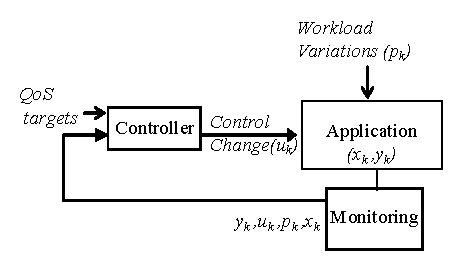
\includegraphics[width=0.45\textwidth]{image/loop/control-loop-general.eps}
	\caption{The general architecture of resource allocation controller.}
	\label{fig:control-loop-general}
\end{figure}

\begin{figure}[b]
	\centering
	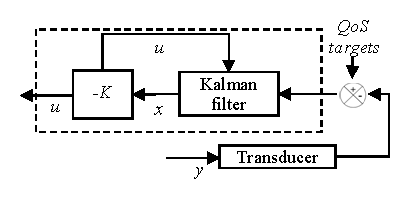
\includegraphics[width=0.45\textwidth]{image/loop/controller-LQG.eps} \label{fig:lqg1}		
	\caption{Structure of an LQG regulator.}  %subref{fig:1}
	\label{fig:lqg}
\end{figure}


For a system whose dynamics are known (e.g. through system identification techniques), a proper feedback based regulator can be constructed at design time using the design techniques such as pole placement, root locus, or etc. 
Dynamics of a system can be represented in several mathematical forms such as transfer functions, state-space models, difference equations, etc; depending on the form used the controller might be designed using the same mathematical method (e.g. a transfer function). 
In several examples, classical linear continuous proportional-integral (PI) and proportional-integral-derivative (PID) controllers are applied to
processor power management \cite{lu2002control,sharma2003power},
QoS adaptation in web servers  \cite{abdelzaher_performance_2002},
and load balancing \cite{hellerstein2004feedback,lu2002aqueduct,parekh2002using}. 
% As an example, consider ....%helesrstin stuf ....

The controller component can also include an estimator that dynamically adjusts the controller gain using the state estimates of the model. For example, Linear-Quadratic-Gaussian (LQG) control (see Figure \ref{fig:lqg}) dynamically adjusts LQ-optimal gain based on a \textit{state estimate} that is used to form a control signal. The estimator is usually a simple or extended Kalman filter~\cite{welch_introduction_1995} able to maintain a good estimate of model unknowns by calibrating itself to the measurements during runtime.
As an example, \cite{kalyvianaki_self-adaptive_2009} tries find the proper CPU share $a_k$ for a VM that satisfies the headroom principal.  
In this case 
%although the system's behavior composed of variations in CPU usage (or utilization) $u_k$ is unknown with respect to inputs: $u_k=u_k+v_k$ ($v_k$ is random step) 
the controller tries to maximize the likelihood that $u_k=60\% a_k + w_k$ (where $u_k$ is CPU utilization and $w_k$ is the random perturbation) by adjusting $a_k$ based on the estimation error $e_k = u_k-60\% a_k$. % That is the controller is itself a Kalman filter with state equation $a_k=a_k+v'_k$ in which the allocation signal $a_k$ is a tracked state variable.

\section{Other ways of implementing managers}
\label{sec:heuristic-regulators}
Although in this chapter we focused on a specific way to implement autonomic managers, there exists several other ways as well.
The description and comparison of these approaches in terms of applicability to problems of different domains, ease of adoption, and ease of learning by humans although interesting, is out of the scope of this report. Here, we only briefly mention a commonly known approach known as policy based autonomic management. 

\subsection{Policy based autonomic management }
Policies are a way of providing ``formal behavioral guides'' to systems about potential actions improving the system's behavior~\cite{KephartEtAlPolicy2004}. 
Policy based management (PBM) is usually used in systems with several components while each component behaves according to the policies passed to it. 
It is used where there is a need for independence in components, either because consulting with central controller on every action is impossible or costly (assume a router that asks for destination of a packet on every arrival) or because components or are prepackaged with certain controllable behavior through predefined policies (i.e. Policy Enforcement Points or PEPs). 

PBM covers a broad spectrum from 
security models (i.e. control access, confidentiality, an integrity)
to network management (routing, traffic flow,  etc),
and computer systems configuration (server configuration). 
There are also several policy description languages (i.e. Imperial College's Ponder, Bell Labs PDL\footnote{Policy Description Language}, IETF's  PCIM\footnote{Policy Core Information Model}, IBM's PMAC\footnote{Policy Management for Autonomic Computing} and ACPL~\footnote{Autonomic Computing Policy Language}).

Policy can be specified different levels of abstraction.
% 
% At the highest level are utility function policies, which specify the relative desirability of
% alternative states. Utility functions are even more powerful than goal policies
% because they automatically determine the most valuable goal in any given situa
Goal policies, describe the conditions to be attained without specifying how to attain them. In business driven policy management, goal policies might target the long term high level business objectives (e.g. minimizing cost and satisfying performance constraints~\cite{Sauve2005}). 
Goal policies  can be refined into operational or action policies for components ~\cite{beigi-policy-transformation,linying-automated}. 
Action policies target real time reactive short term control of systems. 
A low level action policy is usually in the form of event-action rules~\cite{desertot_autonomic_2005,chieu2009dynamic,zhang2010integrating}. 
For example, in an event of 'saturation of component', the action might be 'adding more capacity to X'. 
% (See this being applied to heterogeneous components \cite{garlan2004rainbow,efstratiou2002utilising}).
Event can be a violation of a constraint on certain properties of the configuration or value(s) of monitored metric(s)
(e.g., CPU utilization of an individual VM instance is less than 20 for 10 minutes).
\footnote{A constraint violation may be caused by multiple triggering problems. Thus a condition can be a conjunction or disjunction of other conditions}. 
Note that an implicit target exists for the types of  management rules (e.g. individual server). 
The action part of the rule can be however more complex, including a tactic determination procedure which 
chooses a set of actions to be executed % \cite{gu2002scalable, raman2003policy}). 
Further, an ``action'' might, involve the realization of a global management decision (e.g. adding or removing servers), a local management decision  (e.g. increasing a process's memory), or emitting an event (e.g.,  an {\it alert}). 
See this scheme applied to autoscaling~\cite{rightscale_autoscaling,moreno-elastic-2009}).

In conclusion, policy based techniques are a way to implement the same concept as feedback and feed-forward control, but using a more natural construct for humans to understand which results in ease of use and adoption. This, however, comes with the cost of losing some rigor. Optimality, a criteria usually targeted by control based approaches, cannot necessarily be achieved using policy sets of certain type. Thus, other techniques for policy set optimizations (at design time or runtime) have already been suggested \cite{simmons-strategy-2008,JRLoyolaEtAlCM2006,beigi-policy-transformation}
% 
% Traditionally action policies were specified, edited, and administered by administrators. 
% % In autonomic computing using PBM, intead of a human administrator, an autonomic manager 
% Goal-driven techniques aim at dscovering low level policies from high level ones.
% % Goal Elaboration Using Event-calculus and Abductive Reasoning
% % Goal Elaboration Using Translation Primitives (2006)
% % Policy Optimization (2007)
% 
% 
% %  Using rule bases as a substitute for robust control theory, was first introduced in fuzzy systems.  
% An architecture for a rule-based autoscaler is presented in Figure \ref{fig:rule-based-resource-provisioner}.
% Up to now, solutions to many classic control problems (e.g. 'inverted pendulum' experiment) and real world ones (e.g. camera autofocus and energy-efficient motors) has been implemented using these fuzzy rule based control techniques (e.g. \cite{bevilacqua2007soft,fuzzy_jess_examples}).
%In context of resource provisioning, rule-based systems look promising, because they might be able to scrap the need for complicated full MAPE cycle (i.e. modeling, estimation, forecasting, and control) by simply launching or terminating server resources based on different predefined heuristic conditions (i.e. alerts). 
% according to \cite{dubois_representation_2003} one can emulate more complex probabilistic or fuzzy rules using a large collection of crisp rules. 

% Cfengine provides an autonomous agent and a middle- to high-level policy language for building expert systems which administer
% and configure large computer systems \cite{burgess1995site}

\begin{figure}[tbh]
	\centering
	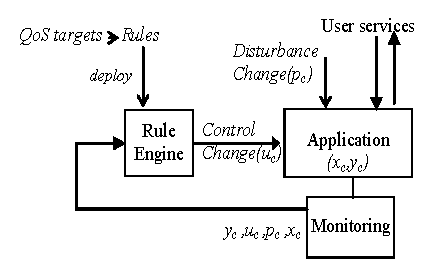
\includegraphics[width=0.45\textwidth]{image/feedback_rule_based.eps} 	
	\caption{Architecture of a rule-based autoscaler.}
	\label{fig:rule-based-resource-provisioner}
\end{figure}

% +++++++++++++++++++
% Application/service adaptation using rule-based techniques was systematically studied in Accord and applied to objects \cite{liu_accord:programming_2006-2} , components \cite{liu2004component , parashar2005conceptual} and
% Grid services [22]
% 
% RESAS \cite{bihari1991dynamic} supports dynamic rule-based adaptation of real-time software and provides tools for programmers.
% 
% ++++++++++++++

% There are various ways that one can configure an autoscaler. 
% For example, in a transactional application deployment with $l$ hosts, $m$ available metrics, and $n$ predicates for defining conditions,
%  each host might choose a subset of $[\text{predicates} \times \text{metrics}]$ (i.e. $2^{n*m}$ choices) to define its alerts.
% These alternatives, together with global configuration parameters \textit{decision threshold}, \textit{resize number}, \textit{min\_instances}, and \textit{max\_instances} form a huge configuration space and this makes it hard to investigate the effect of each configuration parameter on behavior of the autoscaler.    
% % With several tests we concluded a simple scheme for describing the effect each parameter, however. 
% %We considered autoscaler as a transfer function which takes the workload function and maps it to a function representing number of active instances over time (lets call it \textit{node curve}). We also assumed there is only one subsystem under autoscaling (e.g. application servers) with homogeneous instance types. 
% To qualitatively categorize the effect of each configuration parameter on behavior of the autoscaler
% we limited configuration space to a single alert type based on CPU utilization. 
% In our tests all the alerts in all targets were identical and based on the example introduced in Table \ref{tab:alerts-spec-example}, that is, two alerts where defined, one for scale-up action is case of overutilization and one for scale-down in case of under-utilization.
% Overutilization is considered when CPU idle time is less than the lower bound \textit{cpu-idle-lb} and underutilization is defined as when CPU idle time is more than the upper bound \textit{cpu-idle-ub}.
% The interval $[\text{\textit{cpu-idle-ub}},\text{\textit{cpu-idle-ub}}]$ formed by these two bounds, together with decision threshold, refractory period, decision durations, resize numbers, and $[\text{min\_instances},\text{max\_instances}]$ interval form a simpler configuration space that we investigate in this work. 
% We summarized the effect of different autoscaler configurations on the scaling behavior as follows:



